%! TeX program = lualatex
\documentclass[12pt,a4paper]{article}

\usepackage[nil]{babel}
\usepackage{unicode-math}
\usepackage[svgnames]{xcolor}
\usepackage{lmodern}
\usepackage{graphicx}
\usepackage{wrapfig}
\usepackage{float}
\usepackage{parskip}

\babelprovide[import=el, main, onchar=ids fonts]{greek} % can also do import=el-polyton
\babelprovide[import, onchar=ids fonts]{english}

\babelfont{rm}
          [Language=Default]{Liberation Sans}
\babelfont[english]{rm}
          [Language=Default]{Liberation Sans}
\babelfont{sf}
          [Language=Default]{Liberation Sans}
\babelfont{tt}
          [Language=Default]{Liberation Sans}

%Enter Title Here
 \title{Robustness-diagrams-v0.2 \\ LibShare}
\author{\textbf{Ονόματα / ΑΜ / Έτος:} \\ Γρηγόρης Καπαδούκας / 1072484 / 4\textdegree \\ Χρήστος Μπεστητζάνος / 1072615 / 4\textdegree \\ Νικόλαος Αυγέρης / 1067508 / 5\textdegree \\ Περικλής Κοροντζής / 1072563 / 4\textdegree}

\begin{document}

\makeatletter
\begin{center}
	\LARGE{\@title} \\
	\pagebreak
    \begin{LARGE}\@author\end{LARGE}
    \pagebreak
\end{center}

%Insert Body Here
\section{Robustness Diagrams}

\subsection{Αναζήτηση βιβλίων / χρήστη / αιτήσεων}
\begin{figure}[H]
	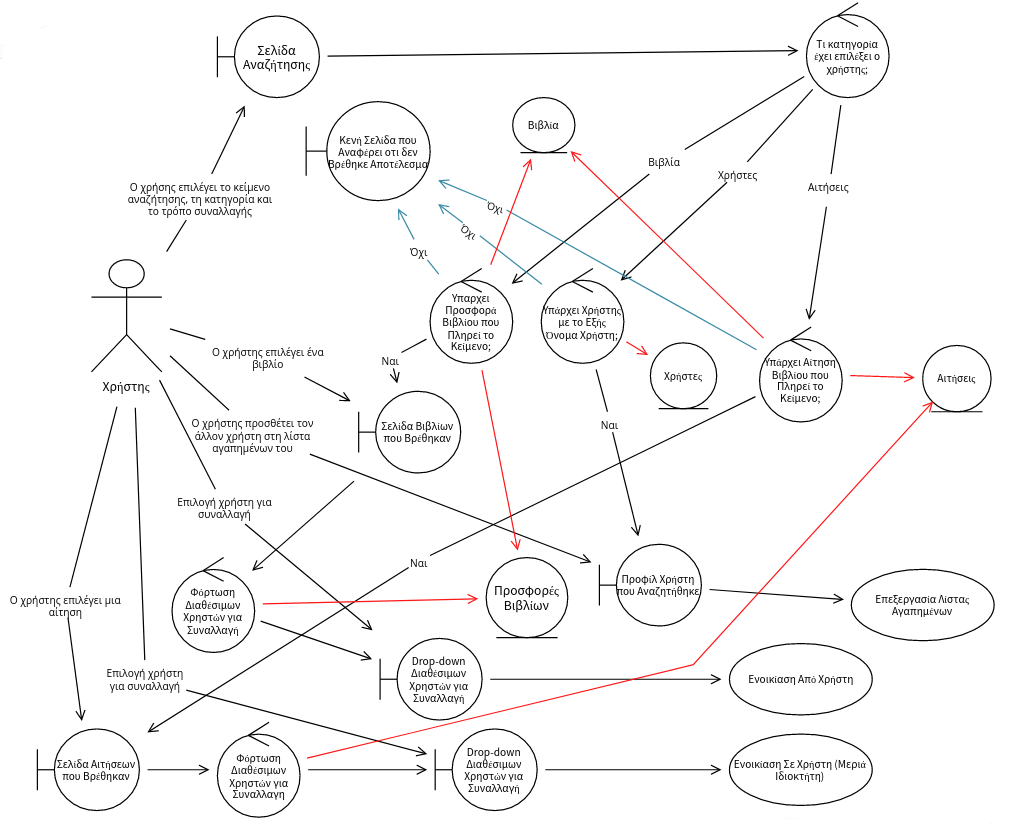
\includegraphics[width=\textwidth]{Search Robustness.png}
	\caption{Robustness Diagram: Αναζήτηση βιβλίων / χρήστη / αιτήσεων}
	\label{Robustness Diagram: Αναζήτηση βιβλίων / χρήστη / αιτήσεων}
\end{figure}

\subsection{Αποδοχή Προσφοράς Βιβλίου και Ενοικίαση}
\begin{figure}[H]
	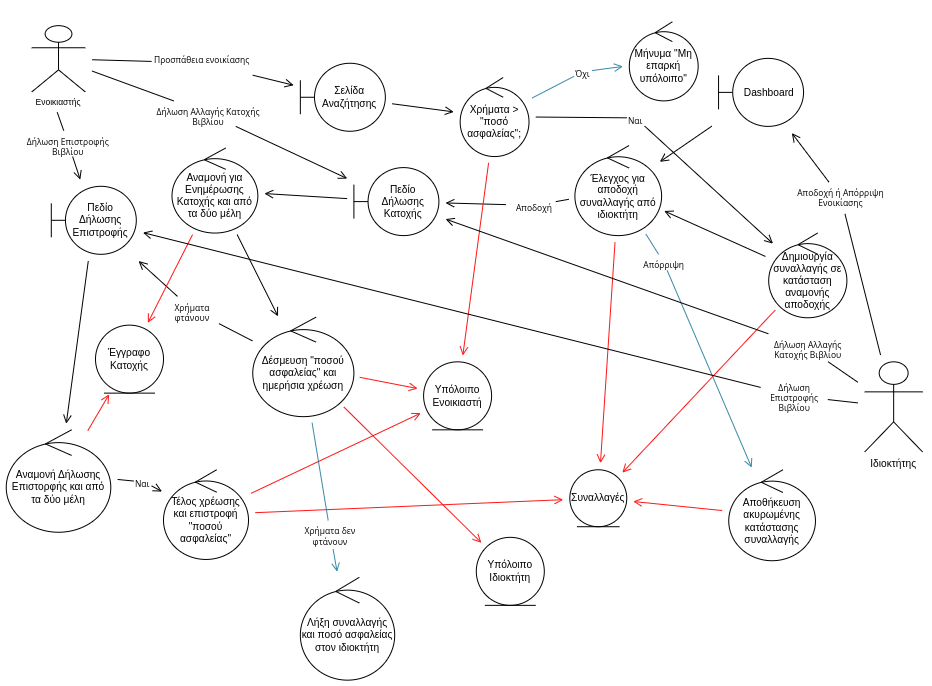
\includegraphics[width=\textwidth]{Accept Book Offer and Rent Robustness.png}
	\caption{Robustness Diagram: Αποδοχή Προσφοράς Βιβλίου και Ενοικίαση}
	\label{Robustness Diagram: Αποδοχή Προσφοράς Βιβλίου και Ενοικίαση}
\end{figure}

\subsection{Αποδοχή Αίτησης Βιβλίου και Ενοικίαση}
\begin{figure}[H]
	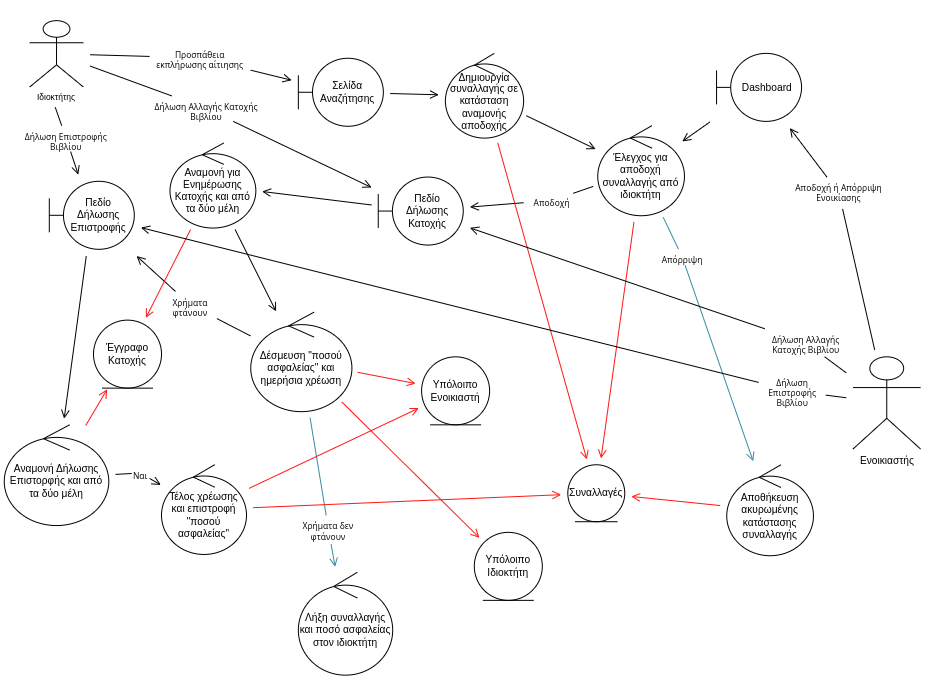
\includegraphics[width=\textwidth]{Accept Request Offer and Rent Robustness.png}
	\caption{Robustness Diagram: Αποδοχή Αίτησης Βιβλίου και Ενοικίαση}
	\label{Robustness Diagram: Αποδοχή Αίτησης Βιβλίου και Ενοικίαση}
\end{figure}

\subsection{Διαχείριση των βιβλίων που προσφέρει ο χρήστης προς ενοικίαση από άλλους}
\begin{figure}[H]
	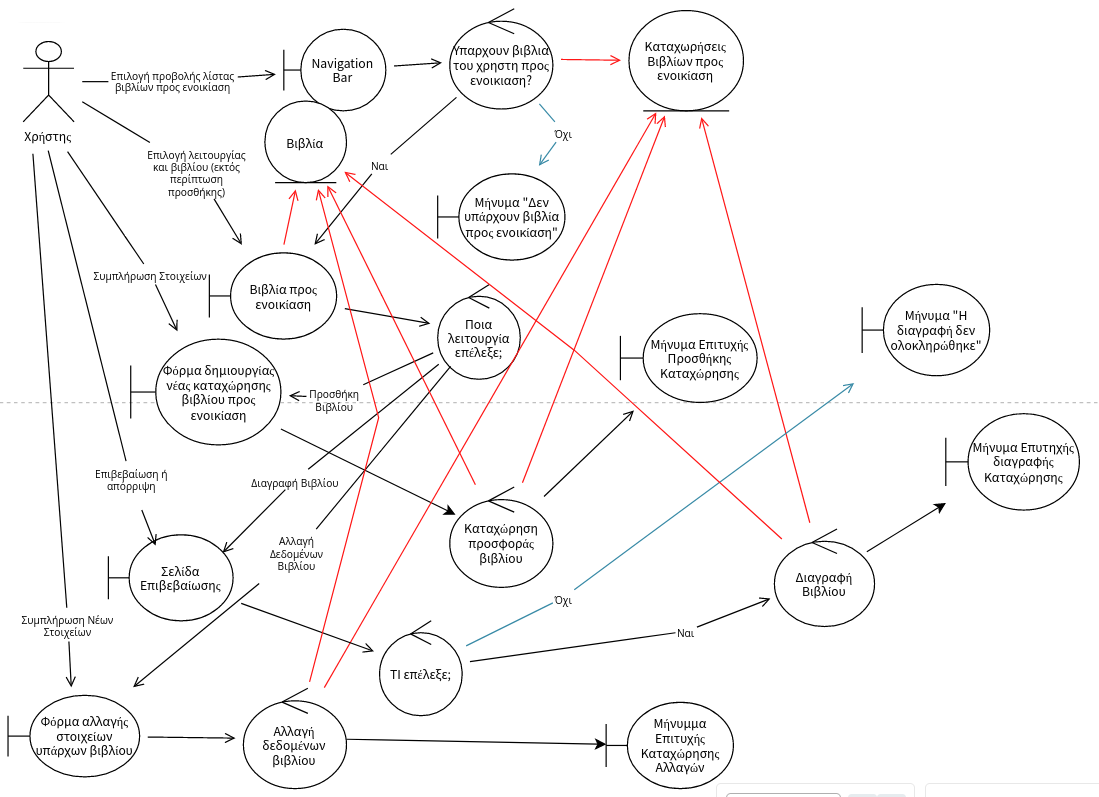
\includegraphics[width=\textwidth]{Manage User Book Listings Robustness.png}
	\caption{Robustness Diagram: Διαχείριση των βιβλίων που προσφέρει ο χρήστης προς ενοικίαση από άλλους}
	\label{Robustness Diagram: Διαχείριση των βιβλίων που προσφέρει ο χρήστης προς ενοικίαση από άλλους}
\end{figure}

\subsection{Διαχείριση των αιτήσεων που έχει κάνει ο χρήστης}
\begin{figure}[H]
	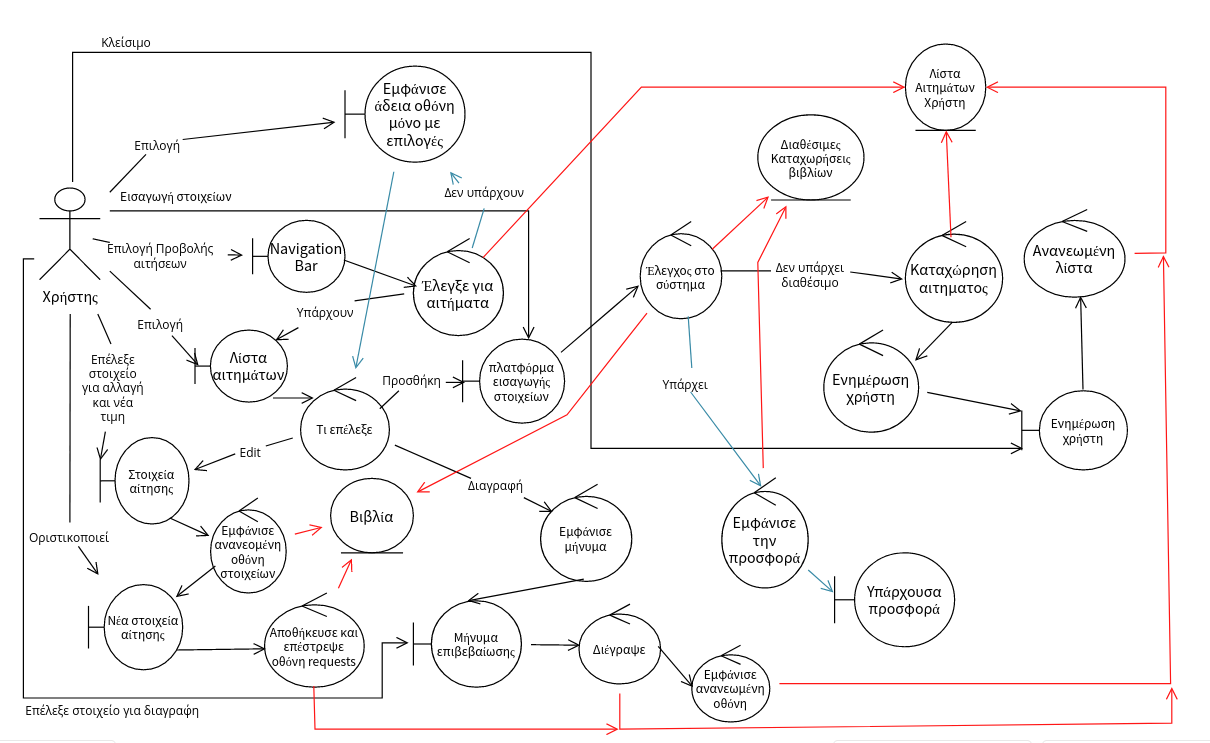
\includegraphics[width=\textwidth]{Manage User Requests Robustness.png}
	\caption{Robustness Diagram: Διαχείριση των αιτήσεων που έχει κάνει ο χρήστης}
	\label{Robustness Diagram: Διαχείριση των αιτήσεων που έχει κάνει ο χρήστης}
\end{figure}

\subsection{Αξιολόγηση άλλων χρηστών μετά από την ολοκλήρωση συναλλαγής}
\begin{figure}[H]
	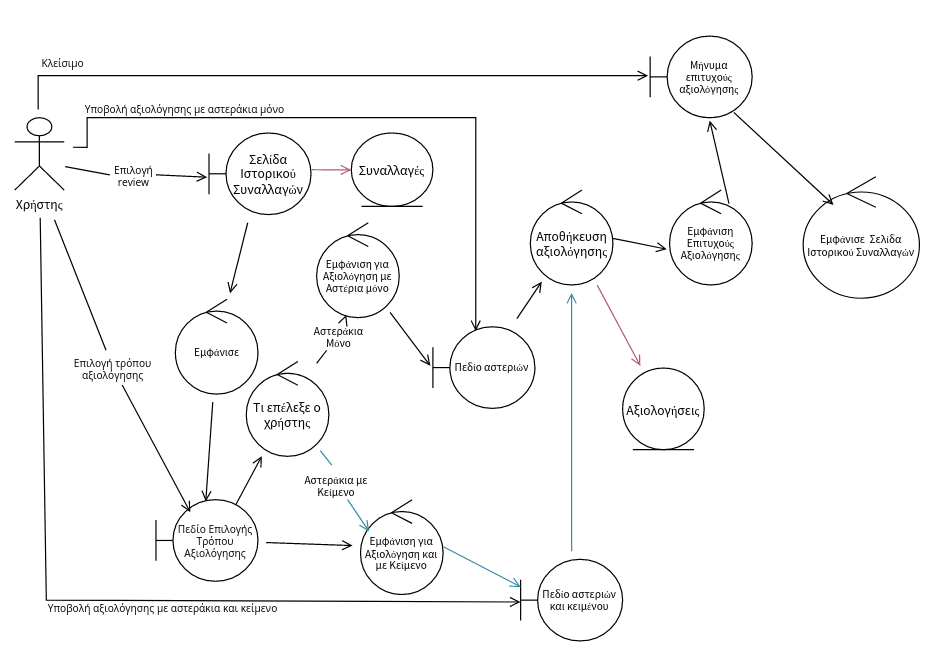
\includegraphics[width=\textwidth]{Review after Transaction Robustness.png}
	\caption{Robustness Diagram: Αξιολόγηση άλλων χρηστών μετά από την ολοκλήρωση συναλλαγής}
	\label{Robustness Diagram: Αξιολόγηση άλλων χρηστών μετά από την ολοκλήρωση συναλλαγής}
\end{figure}


\subsection{Προβολή και Επεξεργασία στοιχείων λογαριασμού χρήστη}
\textbf{Σημείωση:} Στο διάγραμμα αυτό τα δύο boundary objects "Οθόνη Προφίλ με Δυνατότητα Επεξεργασίας" και "Οθόνη προφίλ με ανανεωμένα στοιχεία" αναφέρονται στην ίδια οθόνη, πριν και μετά την αλλαγή αντίστοιχα. Ο λόγος που τα βάλαμε ξεχωριστά είναι για να φαίνεται η αλληλουχία των πράξεων.
\begin{figure}[H]
	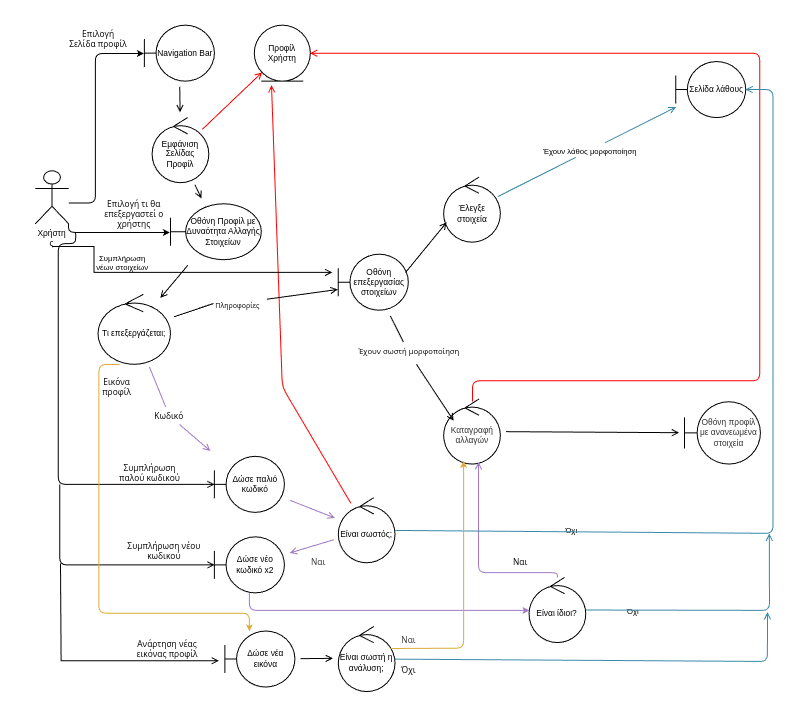
\includegraphics[width=\textwidth]{View and Edit User Account Details Robustness.png}
	\caption{Robustness Diagram: Προβολή και Επεξεργασία στοιχείων λογαριασμού χρήστη}
	\label{Robustness Diagram: Προβολή και Επεξεργασία στοιχείων λογαριασμού χρήστη}
\end{figure}

\subsection{Επεξεργασία χρηματικού υπολοίπου χρήστη}
\begin{figure}[H]
	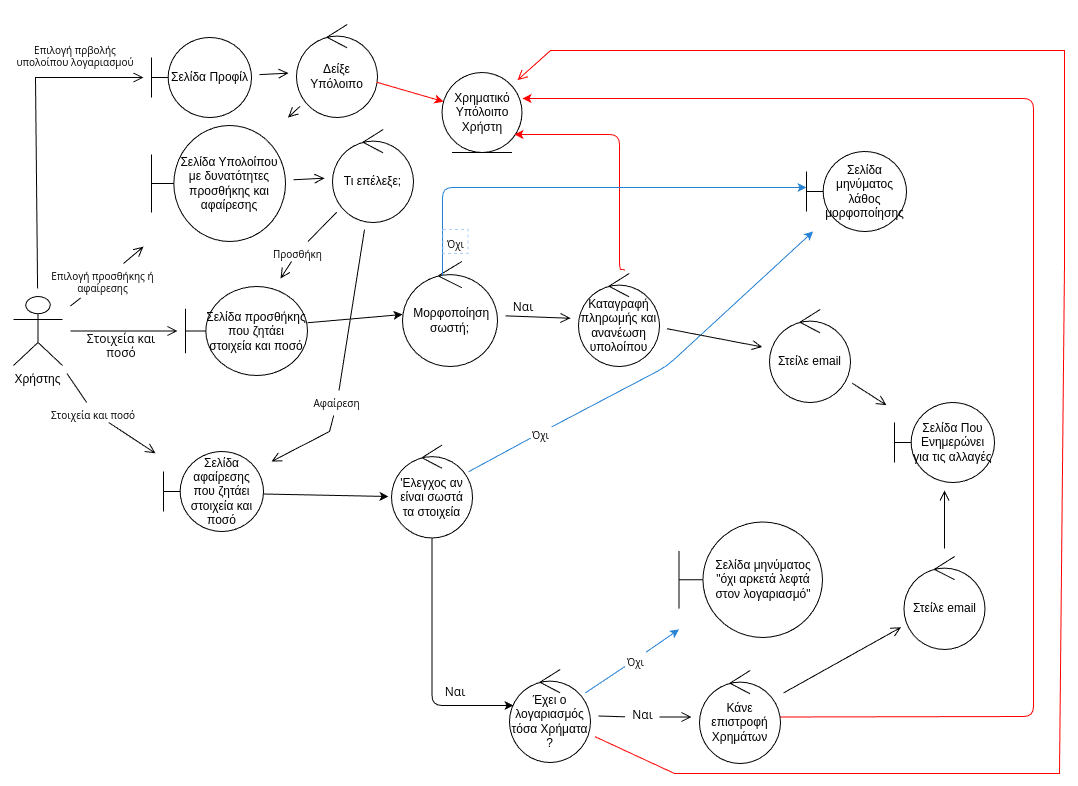
\includegraphics[width=\textwidth]{Edit User Balance Robustness.png}
	\caption{Robustness Diagram: Επεξεργασία χρηματικού υπολοίπου χρήστη}
	\label{Robustness Diagram: Επεξεργασία χρηματικού υπολοίπου χρήστη}
\end{figure}

\subsection{Επεξεργασία λίστας αγαπημένων και χρήση συστήματος ειδοποιήσεων}
\begin{figure}[H]
	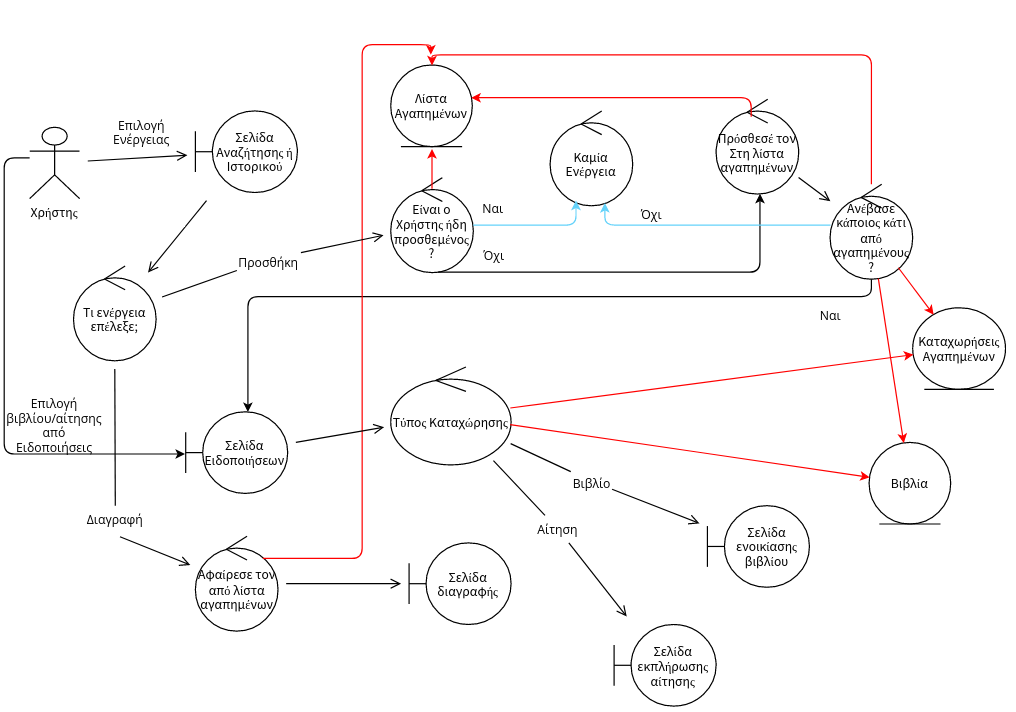
\includegraphics[width=\textwidth]{Favorite Users and Notification System Robustness.png}
	\caption{Robustness Diagram: Επεξεργασία λίστας αγαπημένων και χρήση συστήματος ειδοποιήσεων}
	\label{Robustness Diagram: Επεξεργασία λίστας αγαπημένων και χρήση συστήματος ειδοποιήσεων}
\end{figure}

\subsection{Προβολή ιστορικού συναλλαγών και στατιστικών}
\begin{figure}[H]
	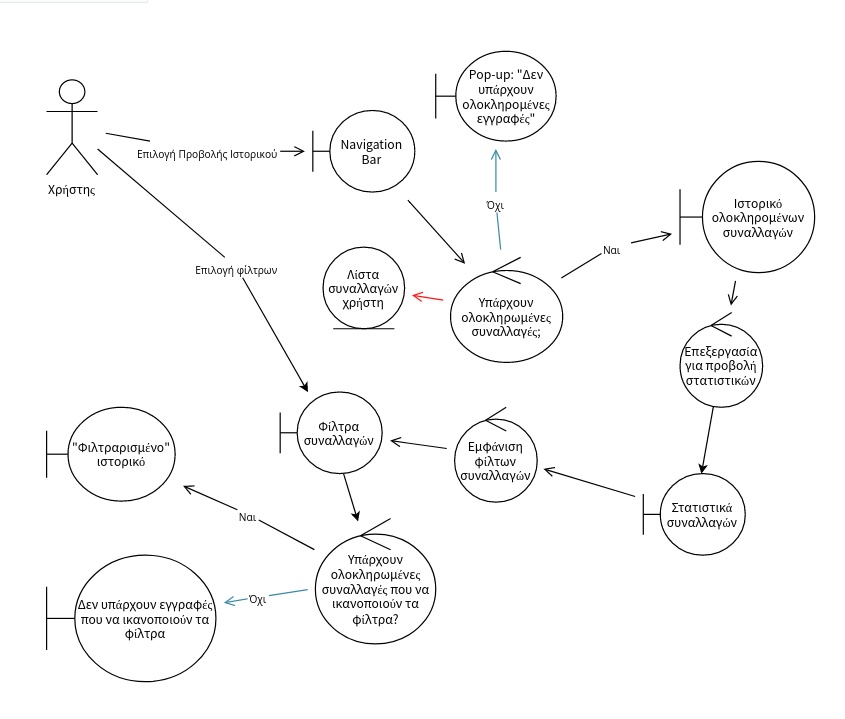
\includegraphics[width=\textwidth]{History and Statistics Robustness.png}
	\caption{Robustness Diagram: Προβολή ιστορικού συναλλαγών και στατιστικών}
	\label{Robustness Diagram: Προβολή ιστορικού συναλλαγών και στατιστικών}
\end{figure}

\section{Συμμετοχή και Ρόλοι στη Συγγραφή του Κειμένου}
\begin{enumerate}
	\item \textbf{Γρηγόρης Καπαδούκας:} Author (Κεφαλαίων 1.1, 1.2, 1.3), Editor Όλων, Reviewer Όλων
	\item \textbf{Χρήστος Μπεστητζάνος:} Author (Κεφαλαίων 1.5, 1.6)
   	\item \textbf{Νικόλαος Αυγέρης:} Author (Κεφαλαίων 1.7, 1.8, 1.9)
	\item \textbf{Περικλής Κοροντζής:} Author (Κεφαλαίων 1.4, 1.10)
\end{enumerate}

\section{Αλλαγές από έκδοση σε έκδοση}

\subsection{Από έκδοση v0.1 σε έκδοση v0.2}
\begin{itemize}
    \item Αλλαγή στο Robustness Diagram για "Αναζήτηση βιβλίων / χρήστη / αιτήσεων".
    \item Διαγραφή των Robustness Diagrams για "Αναζήτηση βιβλίων / χρήστη / αιτήσεων" και "Ενοικίαση βιβλίου από άλλο χρήστη" και αντικατάστασή τους με τα αντίστοιχα για "Αποδοχή Προσφοράς Βιβλίου και Ενοικίαση" και "Αποδοχή Αίτησης Βιβλίου και Ενοικίαση".
    \item Ανανέωση του Robustness Diagram για "Επεξεργασία χρηματικού υπολοίπου χρήστη".
    \item Ανανέωση του Robustness Diagram για "Επεξεργασία λίστας αγαπημένων και χρήση συστήματος ειδοποιήσεων".
    \item Ανανέωση του Robustness Diagram για "Προβολή και Επεξεργασία στοιχείων λογαριασμού χρήστη".
    \item Ανανέωση του Robustness Diagram για "Διαχείριση των βιβλίων που προσφέρει ο χρήστης
προς ενοικίαση από άλλους".
    \item Διόρθωση λάθος αρίθμησης κεφαλαίων στο Κεφάλαιο 2.
\end{itemize}

\end{document}
